%%%%%%%%%%%%%%%%%%%%%%%%%%%%%%%%%%%%%%%%%%%%%%%%%%%%%%
%
% This file defines the style for your report.
%
% Just run "sh compiletex.sh" to compile
% 
%%%%%%%%%%%%%%%%%%%%%%%%%%%%%%%%%%%%%%%%%%%%%%%%%%%%%%

\documentclass[10pt,  english, makeidx, a4paper, titlepage, oneside]{book}
\usepackage{babel}
\usepackage{fancyhdr}
\usepackage{makeidx}
\usepackage{titlesec}
\usepackage{listings}
\usepackage{booktabs}
\usepackage{hyperref}

\newenvironment{listato}{\footnotesize}{\normalsize }

\textwidth 15.5cm
\textheight 23cm
\topmargin -1cm
\oddsidemargin -0.5cm
\linespread{1.1}

\pagestyle{fancy}
\lhead{}
\chead{Cybersecurity for Embedded Systems}
\lfoot{}
\cfoot{}
\rfoot{}
\rhead{\thepage}

\usepackage{graphicx}
\usepackage{amsmath}
\usepackage{amsfonts}
\usepackage{amsthm}
\usepackage{amssymb}
\usepackage{graphicx}
\usepackage{caption}
\usepackage{float}
\usepackage{amsmath}
\usepackage{amssymb}
\usepackage{amsfonts}
\usepackage{amsthm}
\usepackage{empheq}
\usepackage{verbatim}
\usepackage{fancyvrb}
\usepackage{xcolor}
\usepackage{url}
\usepackage{amsmath}  % for \hookrightarrow
\usepackage{xcolor}   % for \textcolor
\definecolor{mGreen}{rgb}{0,0.6,0}
\definecolor{mGray}{rgb}{0.5,0.5,0.5}
\definecolor{mPurple}{rgb}{0.58,0,0.82}
\definecolor{backgroundColour}{rgb}{0.95,0.95,0.92}

\newcommand\clearrow{\global\let\rowmac\relax}
\usepackage{graphicx}

\definecolor{Red}{rgb}{1,0.7,0.7}
\definecolor{Yellow}{HTML}{FAFAD2}
\definecolor{Green}{HTML}{9ACD32}
\definecolor{Blue}{rgb}{0.5,0.8,1}

\lstdefinestyle{CStyle}{
	backgroundcolor=\color{backgroundColour},   
	commentstyle=\color{mGreen},
	keywordstyle=\color{magenta},
	numberstyle=\tiny\color{mGray},
	stringstyle=\color{mPurple},
	basicstyle=\footnotesize,
	breakatwhitespace=false,         
	breaklines=false,                 
	captionpos=b,                    
	keepspaces=true,                 
	numbers=left,                    
	numbersep=5pt,                  
	showspaces=false,                
	showstringspaces=false,
	showtabs=false,                  
	tabsize=2,
	language=C
}
\lstset{basicstyle=\ttfamily,
	showstringspaces=false,
	commentstyle=\color{red},
	keywordstyle=\color{blue},
	postbreak=\mbox{\textcolor{red}{$\hookrightarrow$}\space},
}


\usepackage{graphicx}
\definecolor{Red}{rgb}{1,0.7,0.7}
\definecolor{Yellow}{HTML}{FAFAD2}
\definecolor{Green}{HTML}{9ACD32}
\definecolor{Blue}{rgb}{0.5,0.8,1}
\lstset{
	backgroundcolor=\color{backgroundColour},   
	commentstyle=\color{mGreen},
	keywordstyle=\color{magenta},
	numberstyle=\tiny\color{mGray},
	stringstyle=\color{mPurple},
	basicstyle=\footnotesize,
	breakatwhitespace=false,         
	breaklines=false,                 
	captionpos=b,                    
	keepspaces=true,                 
	numbers=left,                    
	numbersep=5pt,                  
	showspaces=false,                
	showstringspaces=false,
	showtabs=false,                  
	tabsize=2,
	frame=single,
	xleftmargin=15pt,
	xrightmargin=15pt,
	basicstyle=\ttfamily\small
}


\usepackage{blindtext} 
\usepackage{pifont,mdframed}


% Default fixed font does not support bold face
\DeclareFixedFont{\ttb}{T1}{txtt}{bx}{n}{12} % for bold
\DeclareFixedFont{\ttm}{T1}{txtt}{m}{n}{12}  % for normal

\definecolor{mGreen}{rgb}{0,0.6,0}
\definecolor{mGray}{rgb}{0.5,0.5,0.5}
\definecolor{mPurple}{rgb}{0.58,0,0.82}
\definecolor{backgroundColour}{rgb}{0.95,0.95,0.92}

\lstdefinestyle{CStyle}{
    backgroundcolor=\color{backgroundColour},   
    commentstyle=\color{mGreen},
    keywordstyle=\color{magenta},
    numberstyle=\tiny\color{mGray},
    stringstyle=\color{mPurple},
    basicstyle=\footnotesize,
    breakatwhitespace=false,         
    breaklines=true,                 
    captionpos=b,                    
    keepspaces=true,                 
    numbers=left,                    
    numbersep=5pt,                  
    showspaces=false,                
    showstringspaces=false,
    showtabs=false,                  
    tabsize=2,
    language=C
}

% Custom colors
\definecolor{deepblue}{rgb}{0,0,0.5}
\definecolor{deepred}{rgb}{0.6,0,0}
\definecolor{deepgreen}{rgb}{0,0.5,0}

% Python style for highlighting
\lstdefinestyle{PyStyle}{
    backgroundcolor=\color{backgroundColour},   
    commentstyle=\color{mGreen},
    language=Python,
    basicstyle=\footnotesize,
    morekeywords={self},              % Add keywords here
    keywordstyle=\color{deepblue},
    emph={MyClass,__init__},          % Custom highlighting
    emphstyle=\color{deepred},    % Custom highlighting style
    stringstyle=\color{deepgreen},
    showstringspaces=false,
    numbers=left,                    
    numbersep=5pt,                  
}

\lstset{basicstyle=\ttfamily,
  showstringspaces=false,
  commentstyle=\color{red},
  keywordstyle=\color{blue},
}

\newenvironment{warning}
  {\par\begin{mdframed}[linewidth=2pt,linecolor=red]%
    \begin{list}{}{\leftmargin=1cm
                   \labelwidth=\leftmargin}\item[\Large\ding{43}]}
  {\end{list}\end{mdframed}\par}



\titleformat{\chapter}[display]
{\normalfont\Large\filcenter\sffamily}
{\titlerule[0.5pt]%
\vspace{1pt}
\titlerule
\vspace{1pc}
\LARGE\MakeUppercase{\chaptertitlename} \thechapter
}
{1pc}
{\titlerule
\vspace{1pc}
\Huge}

\makeindex

\begin{document}

\frontmatter
\begin{titlepage}
\vspace{0cm}
\centerline{

\includegraphics[width=6cm]{./logopolitonuovo}} 
\vspace{0.5cm}
\centerline{\LARGE Politecnico di Torino}
\vspace{2.5cm}
\centerline{\huge Cybersecurity for Embedded Systems}
\vspace{0.25cm}
\centerline{\huge 01UDNOV}
\vspace{1cm}
\centerline{\Large Master's Degree in Computer Engineering}
\vspace{2.5cm}
\centerline{\Huge Browser Password Manager}
\bigskip
\centerline{\huge Project Report}
\vspace{2cm}
\vfill
\begin{minipage}{9.5cm} % modify this width in order to keep everything on the same line
\Large{Candidates:\\
Matteo Battilana (281389)\\
Gabriele Salvatore La Greca (281589)} \\
Giovanni Pollo (s290136)\\
\end{minipage}
\hfill
\begin{minipage}{4.4cm}
\Large{Referents: \\
Prof. Paolo Prinetto\\
Dr. Matteo Fornero\\
Dr. Vahid Eftekhari}
\end{minipage}
\end{titlepage}

\tableofcontents
\listoffigures % REMOVE THIS IF THERE ARE NO PICTURES
\listoftables % REMOVE THIS IF THERE ARE NO TABLES

\mainmatter
    
% HERE IS WHERE YOU INCLUDE YOUR CHAPTERS

\chapter*{Abstract}

It is widely known that passwords are becoming more and more important, since every day people are using them to protect their data. There are several ways to store your passwords, such as writing them on a piece of paper or in a file (both in the smartphone or in the laptop). Another method is to remember by hearth the passwords, but this is not feasible since there would be too many pieces of information to remember. In this context, password managers, such as Bitwarden, LastPass, or Keepass, are good solutions. However, if not self-hosted, all these password managers store the passwords in a cloud, which means that they are not completely under the user control. 

These were the main reasons behind the creation of this project, whose goal is to help people to remember their passwords, and to make it easier for them to access their data. In addition to that, data are stored on a board, which is secure by definition thanks to the technology used. Moreover it is needed to have access to the physical board in order to manage the data. 

The password manager has been designed from the ground up to be secure, but it also has a user-friendly Chrome extension that simplifies the insertion of the passwords in various websites.
% \chapter{Generic Chapter}
This is a generic chapter of your thesis. Remember to put ANY chapter in a different source file (including introduction and all the others). 

For the purpose of this guide, the main \LaTeX constructs and how to use them will be explained here. Other thematic chapters will follow, i.e., which will trace the chapters that should be present in your thesis. Delete this generic chapter once you have learned this contents.

You can write in italic \emph{like this}, you can write in bold \textbf{like this}, or you can write using colors \textcolor{cyan}{like this}.

This is an \emph{itemize}, where you can put a list of items, like this:
\begin{itemize}
\item item number 1
\item item number 2
\end{itemize} 

This is an \emph{enumerate}, where you can put a list of items with numbers, like this:
\begin{enumerate}
\item item number 1
\item item number 2
\end{enumerate} 

You can cite references like this: \cite{lee2016introduction} \cite{jiang2013towards}, by using the \lstinline{\cite} directive. You have to copy within \lstinline{\cite} brackets the label of the entry that you have in the BibTeX file (\texttt{.bib}). The \texttt{.bib} file of this thesis is \texttt{mybib.bib}. he command \lstinline{\addbibresource} at the top of this main file indicates what BibTeX file you are referring to. 

As an example, this is a BibTeX entry:

\begin{verbatim}
@inproceedings{urias2018cyber,
  title={Cyber Range Infrastructure Limitations and Needs of Tomorrow: A Position Paper},
  author={Urias, Vincent E and Stout, William MS and Van Leeuwen, Brian and Lin, Han},
  booktitle={2018 International Carnahan Conference on Security Technology (ICCST)},
  pages={1--5},
  year={2018},
  organization={IEEE}
}
\end{verbatim}

For every online paper that you may read on online libraries, you can download its BibTeX entry. For example:
\begin{enumerate}
	\item For IEEE Xplore, click on the paper name, then click on ``Cite This'', ``BibTeX'', and you can find the entry;
	\item For Google Scholar, click on the ``Cite'' voice under the paper name, then click ``BibTeX'', and you can find the entry. 
\end{enumerate}

Just copy and paste such an entry in the .bib file. If you find a paper on Scholar that is nevertheless published by IEEE, by convention you should take the entry from the IEEE website and not from Scholar. To do this, just click on the title of the paper. This will redirect you to the resource page on IEEE Xplore. Once here, follow instructions at point 1.

When you compile, a correct number will automatically be assigned to the citation in the text, and the complete entry will appear at the bottom of the document, in the ``Bibliography'' chapter. 

If you need to cite a generic online resource, which does not necessarily correspond to a scientific paper, use the \lstinline{@misc} entry in the \texttt{.bib} file. A \lstinline{@misc} entry looks like this:

\begin{verbatim}
@misc{nist2018,
    author = "{NIST}",
    title = "Cyber Ranges",
    year = "2018",
    howpublished = "\url{https://www.nist.gov/system/files/documents/2018/02/13/cyber_ranges.pdf}",
    note = "[Online; Accessed 2019, 28 November]"
  }
\end{verbatim}

You have to manually create this entry from scratch and manually type these fields. Remember not to forget any of these fields. You can choose the label with which to refer to the resource. The title of the website (which you can see at the top of the tab of your browser showing the page) can be used as the title of the resource.

In general, enter a citation of this type for sites only when there are data, phrases, or images that you intend to report. Instead, if you want to cite names of software or hardware devices, prefer the use of the \lstinline{\footnote}, in which you will only have to specify the URL of the item. 

Remember that citations, both in the text and in the image captions, usually go to the end of a sentence, before the fullstop, as in this case \cite{vykopal2017kypo}. In case of long periods, they can also be placed before other detachment signs, such as commas or semicolons, or colons if they precede a list, itemized or enumerated. An exemption is allowed in the event that the name of research projects, described in some scientific resource, is being introduced, as in this case:

\begin{center}
Cybertropolis \cite{deckard2018cybertropolis} is described in a very good paper by Gary Deckard.
\end{center}

Remember to put citations very often to justify your claims, especially when you report data or results. Just consider them as a justification of what you, in an original way, are writing. Citations are not needed to have permission to copy and paste sentences from online resources, which should NEVER be done - always try to rephrase the concept with your words.

\begin{figure}[h!]
\vspace{0.5cm}
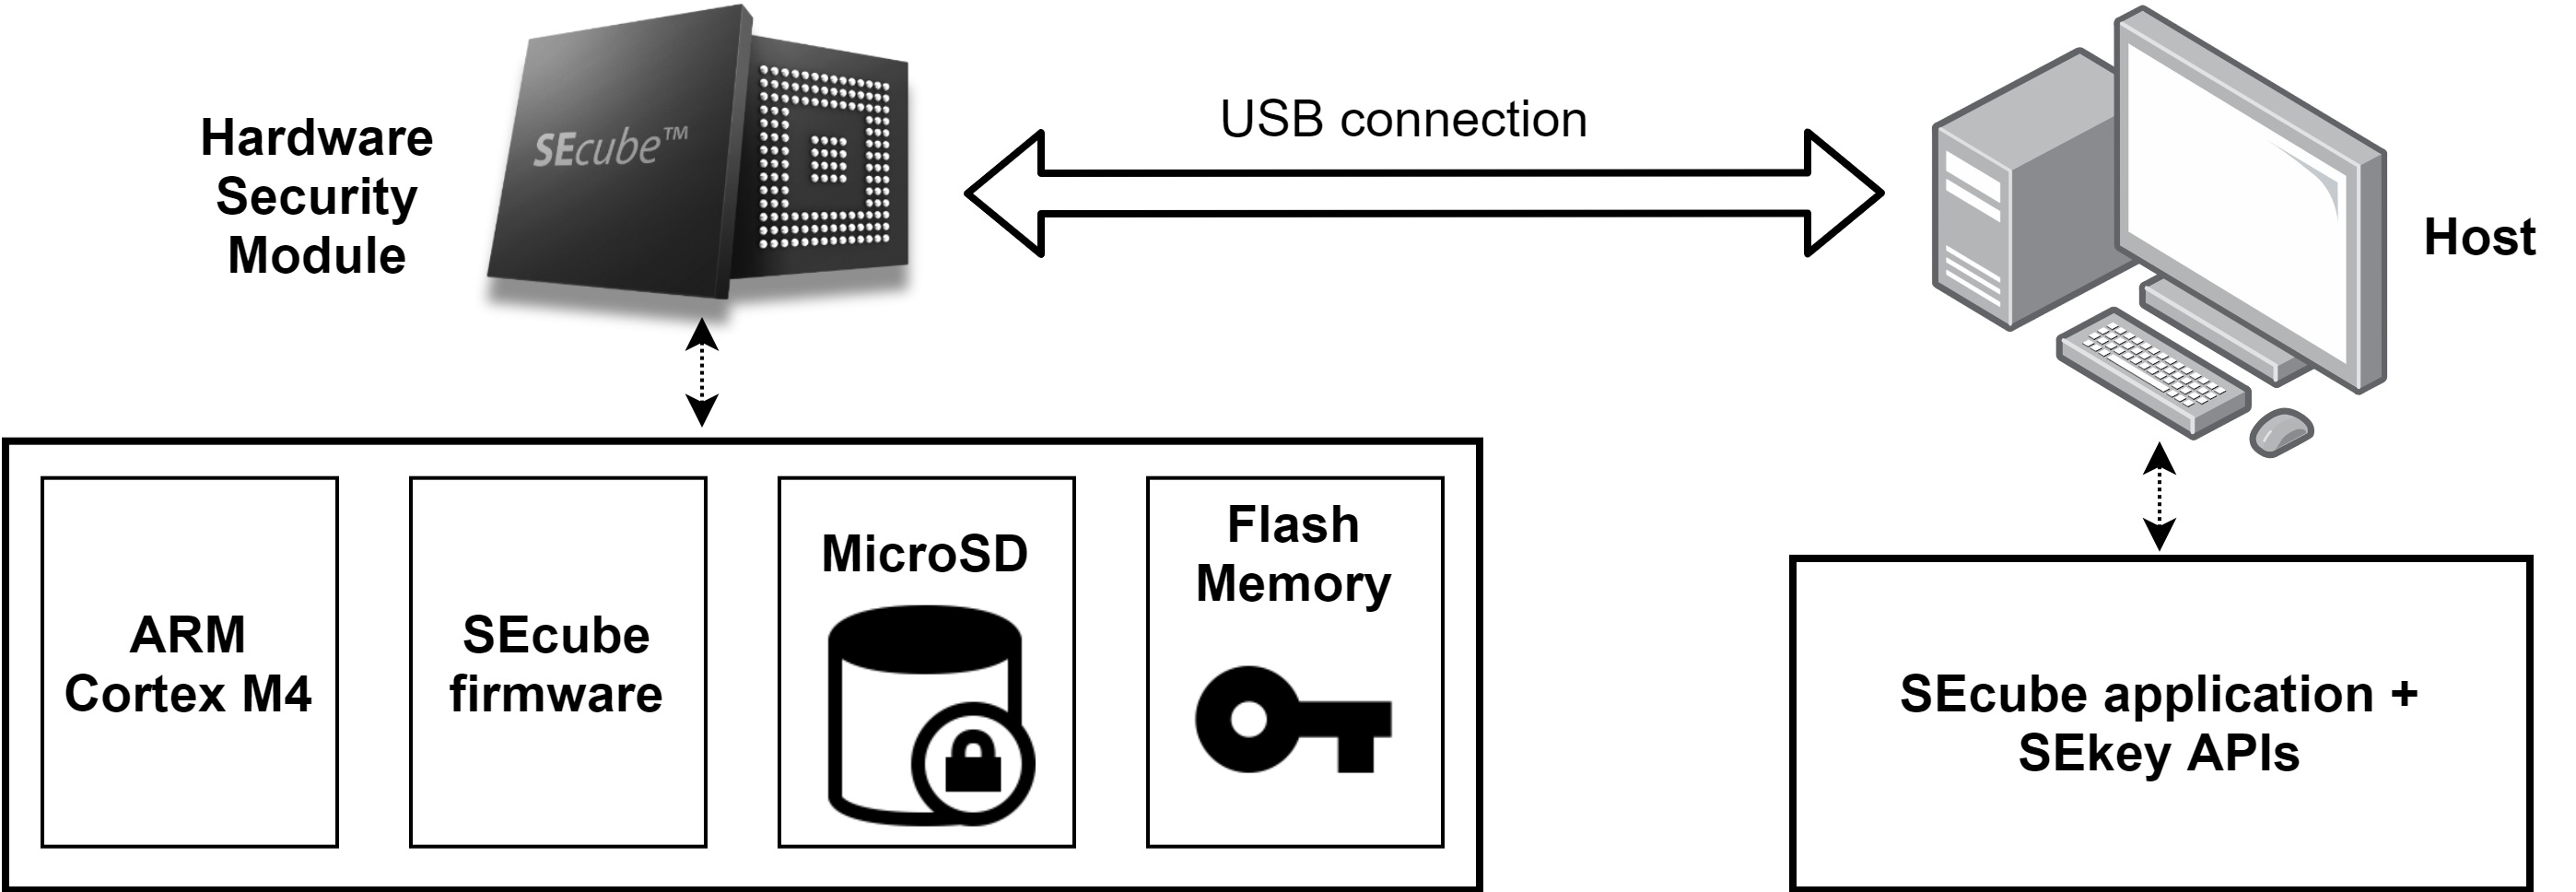
\includegraphics[width=\textwidth]{images/simplearch.jpg}
\caption{This is the image \emph{caption}.}
\label{fig:generalschema} % This is the image label, with which you can refer to the image in any document location.
\end{figure}

This is an image example. Images must ALWAYS be understandable: never introduce images that have text smaller than the text in your document. If you create the images yourself, try not to make them clash too much with the style of your document, and use the same font as this thesis.
If they are not images of your own creation, you MUST reference them. In the caption of the image, you need to insert a citation to the resource from which you took the image, at the end of the caption sentence, before the fullstop.
Each image you enter MUST be referenced in the text, using a formula similar to this:

\begin{center}
Figure \ref{fig:generalschema} describes the architecture of the system.
\end{center}

You can refer to the image using \lstinline{\ref} followed by the image label, that you put in the \lstinline{\label} entry of the figure. Remember to use the word Figure with a capital F. 

Remember that the more your text is adorned with figures, the more understandable, appreciable and readable it becomes.

\section{Section title}\label{examplesection}
This is a section under a chapter. The number of sections also contributes to greater readability of your text, and to a better display of the content in the index. In fact, sections are automatically shown in the Table of Contents. However, try not to make sections shorter than two pages. For smaller portions of your text, use subsections.

You can refer to a section using its label, using the \lstinline{\ref} directive as for images, like this:

\begin{center}
This concept has been explained in Section \ref{examplesection}.
\end{center}

Remember to use the word Section with a capital S. This is also valid for chapters. 

\subsection{Subsection title}
This is a subsection under the section. 

The following is a table.

\begin{table}
\centering
\caption{Preliminary Experimental Results}
\begin{tabular}{| p{3cm} | p{3cm} | p{3cm} |}
    \hline
    \textbf{Benchmark} & \textbf{Inputs} & \textbf{Processing time} \\ \hline
    SHA & Message of 100 KB & 368449 s \\ \hline
    RIJNDAEL & Message of 100 KB & 1083568 s \\ \hline
    DIJKSTRA & Matrix of 100x100 32-bit integers & 324782 s \\ \hline
    STRING & 1331 50-char strings & 178616 s \\ \hline
    BITCOUNT & 12800 32-bit integers & 419545 s \\ \hline
    \hline
\end{tabular}
\label{tab:ar}
\end{table}

If you want to write a formula, you can do like this:

\begin{equation}\label{eq:thiseq}
X_{k}=\sum _{n=0}^{N-1}x_{n}e^{-ik{\frac {2\pi }{N}}n}\quad \quad k=0,\dots ,N-1
\end{equation}

Tables and formulas are extensively documented online, and any doubts about their syntax can be easily resolved with a simple search. As for figures and sections, the same rules also apply to tables and formulas: mandatory reference in the text, possibility to use \lstinline{\label} to label them, and naming with capital letter (e.g., ``as in Table \ref{tab:ar}, as in Formula \ref{eq:thiseq}).

The following is a piece of code:

\begin{lstlisting}
int func(int N, int M) {
  float (*p)[N][M] = malloc(sizeof *p);
  if (!p)
    return -1;
  for (int i = 0; i < N; i++)
    for (int j = 0; j < M; j++)
      (*p)[i][j] = i + j;
  print_array(N, M, p);
  free(p);
  return 1;
}
\end{lstlisting}

You can customize the style of your code, changing the language, the colors of keywords, of comments or the background by changing the settings inside the \lstinline{\lstset} directive found in the main file. Usually, the listings are not referenced within the text as happens for figures, tables, formulas and sections. Do not overdo the code within your text: use it only for short passages (e.g., function prototypes, or 2 to 5 lines of code within a function to help the reader in better understanding the meaning of the text).

You can also write in-text code using the \lstinline{\lstinline} directive, \\
like this: \lstinline{int main(int argc, char** argv);}.


\chapter{Introduction}
%% DELETE THE TEXT BELOW
%In this first chapter we expect you to introduce the project explaining what the project is about, what is the final goal, what are the topics tackled by the project, etc.\newline The introduction must not include any low-level detail about the project, avoid sentences written like: we did this, then this, then this, etc.\newline It is strongly suggested to avoid expressions like `We think`, `We did`, etc...it is better to use impersonal expressions such as: `It is clear that`, `It is possible that`, `... something ... has been implemented/analyzed/etc.` (instead of `we did, we implemented, we analyzed`).\newline In the introduction you should give to the reader enough information to understand what is going to be explained in the remainder of the report (basically, expanding some concept you mentioned in the Abstract) without giving away too many information that would make the introduction too long and boring.\newline Feel free to organize the introduction in multiple sections and subsections, depending on how much content you want to put into this chapter.

%Remember that the introduction is needed to make the reader understand what kind of reading he or she will encounter. Be fluent and try not to confuse him or her.
%The introduction must ALWAYS end with the following formula: The remainder of the document is organized as follows. In Chapter 2, ...; in Chapter 3, ... so that the reader can choose which chapters are worth skipping according to the type of reading he or she has chosen.





\chapter{Background}
\label{sec:background}

\subsection{Password Manager}

A password manager is a computer program that allows users to store, generate, and manage their passwords for local applications and online services.
A password manager assists in generating and retrieving complex passwords, storing such passwords in an encrypted database, or calculating them on demand.

Types of password managers include:

\begin{itemize}
    \item Locally installed software applications
    \item Online services accessed through website portals
    \item Locally accessed hardware devices that serve as keys
\end{itemize}

Depending on the type of password manager used and on the functionality offered by its developers, the encrypted database is either stored locally on the user's device or stored remotely through an online file-hosting service. Password managers typically require a user to generate and remember one ``master" password to unlock and access any information stored in their databases.

\subsection{Locally Installed Software Applications}

Password managers commonly reside on the user's personal computer or mobile device, in the form of a locally installed software application. These applications can be offline, wherein the password database is stored independently and locally on the same device as the password manager software. Alternatively, password managers may offer or require a cloud-based approach, wherein the password database is dependent on an online file hosting service and stored remotely, but handled by password management software installed on the user's device.

Some offline password managers do not require Internet permissions, so there is no leakage of data due to the network. To some extent, a fully offline password manager is more secure, but may be much weaker in convenience and functionality than an online one.


\subsection{Online Services Accessed Through Website Portals}

An online password manager is a website that securely stores login details. They are a web-based version of more conventional desktop-based password manager.

The advantages of online password managers over desktop-based versions are portability (they can generally be used on any computer with a web browser and a network connection, without having to install software), and a reduced risk of losing passwords through theft from or damage to a single PC, although the same risk is present for the server that is used to store the users passwords on. In both cases this risk can be prevented by ensuring secure backups are taken.

The major disadvantages of online password managers are the requirements that the user trusts the hosting site and that there is no keylogger on the computer they are using. With servers and the cloud being a focus of cyberattacks, how one authenticates into the online service and whether the passwords stored there are encrypted with a user defined key are just as important. Another important factor is whether one- or two-way encryption is used.

Some online password management systems, such as Bitwarden, are open source, where the source code can be independently audited, or hosted on a user's own machine, rather than relying on the service's cloud.

\subsection{Locally Accessed Hardware Devices That Serves as Keys}

Token-based password managers need to have a security token mechanism, wherein a locally-accessible hardware device, such as smart cards or secure USB flash devices, is used to authenticate a user. The data stored in the token are usually encrypted to prevent probing and unauthorized reading of the data. Some token systems still require software loaded on the PC along with hardware (smart card reader) and drivers to properly read and decode the data.

Credentials are protected using a security token, thus typically offering multi-factor authentication by combining something the user has such as a mobile application that generates rolling codes, similar to virtual smart card, smart card and USB stick, something the user knows (PIN or password), and/or
something the user is, like biometrics such as a fingerprint, hand, retina, or face scanner.
There are a few companies that make specific third-party authentication devices, with one of the most popular being YubiKey.

\subsection{Chrome Extension}

A browser extension is a small software module for customizing a web browser. Browsers typically allow a variety of extensions, including user interface modifications, cookie management, ad blocking, and the custom scripting and styling of web pages.
The extensions, to allow the user to interact with the browser has been developed using Chrome's WebExtension API, since Google Chrome is the most popular browser in the world. However, since the extension is not embedded in the browser, it can be installed on any browser that is Chromium-based.

\chapter{Implementation Overview}
\label{sec:implementation-overview}

The goal is to develop a secure Password Manager, where passwords are stored in a secure and removable USB device, that is based on SECube. Different challenges need to be solved in order to achieve this goal: from the SECube's firmware to the development of a Chromium Extension. \bigskip

The main problem is the communication between the Chromium Browser and the SECube: due to the high level of restrictions imposed by any modern web browser, indeed they act as a big and complex sandboxes for good reasons, it's nearly impossible to have a direct connection between the Extension and any physical device connected to the Host PC. \bigskip

Because of this, a third actor needs to be introduced: a middleware that is capable of being both interfaced with any (Chromium-based) browser and able to communicate with the SECube device. Thus, the middleware is a third software that is intended to be installed and run on the host PC continuously (like a service on Windows or a daemon on Linux, or executed by the user when he needs it, as he prefers). \bigskip

\section{The solution}

\begin{figure}[H]
	\centering
	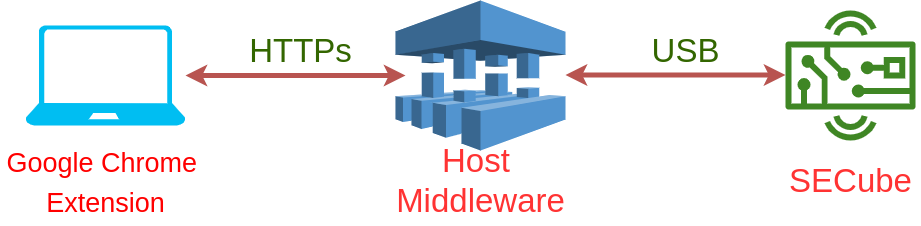
\includegraphics[width=0.9\linewidth]{images/overview}
	\caption{How the three actors interact between each other}
	\label{fig:overview}
\end{figure}

Due to all these actors, developing a secure Password Manager becomes very complicated. It is very important, in cases like this, to be pretty organized and try to be systematic in developing all the needed software, without trying to reinvent the wheel. \bigskip

The three components have been developed completely independent from others one, trying to move all the possible logic and sensitive data to the lowest level (i.e. the Host Middleware and the SECube): this is due to the fact that these two actors are the most secure while the Extension is the most exposed one to possible threats. \bigskip

The communication between the Extension and the Middleware happens by means of HTTPs: it is a secure version of HTTP based on TLS, allowing to have a complete communication between the two parties. The communication between the Middleware and the SECube happens by means of a USB connection, and the communication is encrypted. 

% In this chapter you should provide a general overview of the project, explaining what you have implemented staying at a high-level of abstraction, without going too much into the details. Leave details for the implementation chapter. This chapter can be organized in sections, such as goal of the project, issues to be solved, solution overview, etc.\\It is very important to add images, schemes, graphs to explain the original problem and your solution. Pictures are extremely useful to understand complex ideas that might need an entire page to be explained.\\Use multiple sections to explain the starting point of your project, the last section is going to be the high-level view of your solution...so take the reader in a short `journey` to showcase your work.

\chapter{Implementation Details}
This is where you explain what you have implemented and how you have implemented it. Place here all the details that you consider important, organize the chapter in sections and subsections to explain the development and your workflow.\\Given the self-explicative title of the chapter, readers usually skip it. This is ok, because this entire chapter is simply meant to describe the details of your work so that people that are very interested (such as people who have to evaluate your work or people who have to build something more complex starting from what you did) can fully understand what you developed or implemented.\\Don't worry about placing too many details in this chapter, the only essential thing is that you keep everything tidy, without mixing too much information (so make use of sections, subsections, lists, etc.). As usual, pictures are helpful.
\chapter{Results}
In this chapter we expect you to list and explain all the results that you have achieved. Pictures can be useful to explain the results. Think about this chapter as something similar to the demo of the oral presentation. You can also include pictures about use-cases (you can also decide to add use cases to the high level overview chapter).
\section{Known Issues}
If there is any known issue, limitation, error, problem, etc...explain it in this section. Use a specific subsection for each known issue. Issues can be related to many things, including design issues.
\section{Future Work}
\label{sec:future_work}


\chapter{Conclusions}
\label{sec:conclusions}

This project has been developed to provide the user a secure platform, called Secure Password Manager, in which store and generate passwords via a simple user interface. The entire architecture has been developed following the based principle in order to provide the highest possible level of security but at the same time to not mitigate and reduce the overall usability.\newline\newline
The project is divided into three different modules:
\begin{enumerate}
	\item The SECube provides the secure hardware in which the \textbf{firmware} is running and provides the basic APIs to be handled indirectly from the browser extension but directly from the Host Middleware. It basically provide the functionality to store, retrieve and generate passwords in a secure manner;
	\item In order to allow the extension to communicate with the SECube device, an host \textbf{Middleware} has been developed to expose RESTful APIs in HTTPs in C++ and Python. This allowed to create an obfuscated executable both for Windows and Linux;
	\item The last component is the \textbf{Chrome extension} iteself that allows the user to directly manage all Secure Password Manager functionality; this solution adopts all the needed easy-to-use UI approaches
\end{enumerate}
The system is complete and usable from the user point of view, refer to Section \ref{sec:know_issues} and \ref{sec:future_work} for possible known issues and future work related tasks. All initial and proposed functionalities have been implemented and extensively test to avoid problem visible at the user. 


\begin{thebibliography}{9}
% The bibligraphy is mandatory. Here you have a couple of examples (remember to put references in the text).
\bibitem{texbook}
Donald E. Knuth (1986) \emph{The \TeX{} Book}, Addison-Wesley Professional.

\bibitem{lamport94}
Leslie Lamport (1994) \emph{\LaTeX: a document preparation system}, Addison
Wesley, Massachusetts, 2nd ed.
    
\end{thebibliography}

%%%%%%%%%%%%%%%%%%%%%%%%%%%%%%%%%%%%%%%%%%%%%%%%%%%%%
    
% HERE IS WHERE YOU INCLUDE YOUR APPENDICES (IF ANY)

\appendix
\chapter{User Manual}
\label{usermanual}

\subsection{Firmware}
This tutorial needs a working version of Eclipse for C/C++ and the AC6 Tools are properly installed in order to build the firmware and flash it to the SECube device. The configuration describes uses the following configuration:
\begin{itemize}
	\item ST-Link/v2 programmer
	\item Eclipse IDE for C/C++ Developers (includes Incubating components) Version: 2022-03 (4.23.0) Build id: 20220310-1457
	\item Ubuntu 18.04 5.4.0-117-generic
\end{itemize}

\subsubsection{Hardware and Compiler setup}
In this Section are reported the instructions you need to follow to properly connect the SEcube DevKit to the Host PC and to Programmer/debugger, refer to Figure \ref{fig:setup2}. A more detailed configuration tutorial is available via the  \href{https://github.com/SEcube-Project/SEcube-SDK/blob/master/wiki/wiki_rel_012.pdf}{official SECube Wiki}.

\begin{figure}[H]
	\centering
	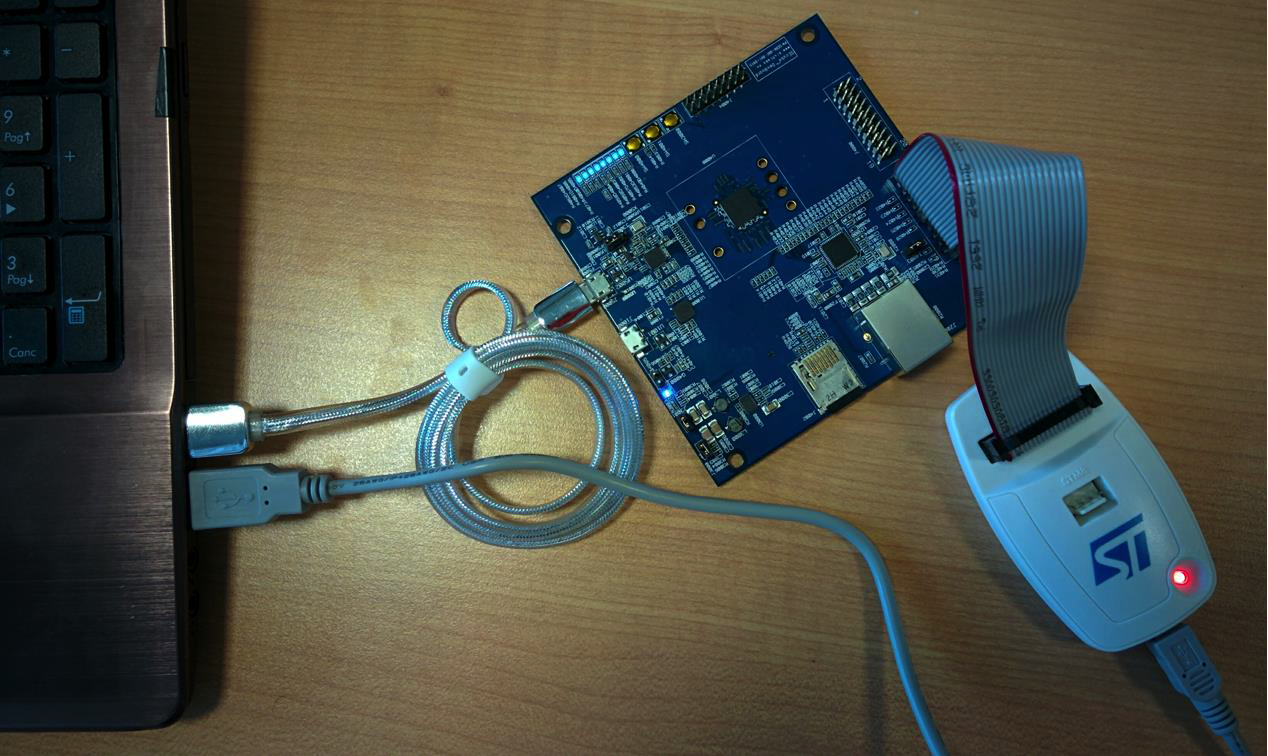
\includegraphics[width=0.42\linewidth]{images/firmware/setup_2}
	\caption{Connection between the STLink/v2 programmer and the SEcube DevKit}
	\label{fig:setup2}
\end{figure}

\begin{figure}
	\centering
	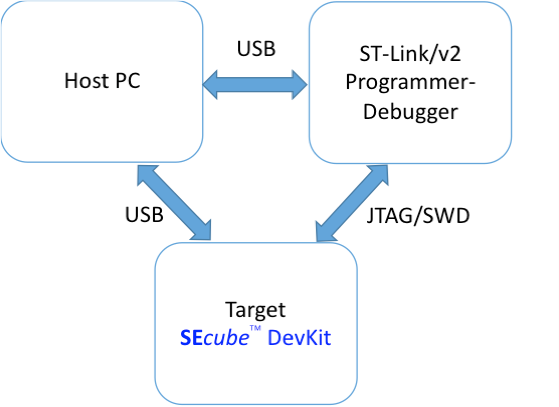
\includegraphics[width=0.35\linewidth]{images/firmware/setup_4}
	\caption{System Architecture}
	\label{fig:setup4}
\end{figure}


Assembling is composed of the following two steps in order to obtain the situation that is available at Figure \ref{fig:setup4}:
\begin{enumerate}
	\item Connect the SEcube DevKit with the programmer by means of the JTAG/SWD cable: the
	cable should be inserted on the JTAG docks on both the programmer (in this case the orientation of the plug is forced from the dock) and the DevKit (in this case you must pay
	attention in inserting the plug on top of both lines of connectors and with its protrusion
	oriented towards the inner side of the DevKit).
	\item Connect the ST-Link/v2 with the PC by means of the USB cable.
\end{enumerate}
The system assembled is shown in Figure \ref{fig:setup2}, while a close-up on the JTAG connection is in Figure \ref{fig:setup3}.

\begin{figure}
	\centering
	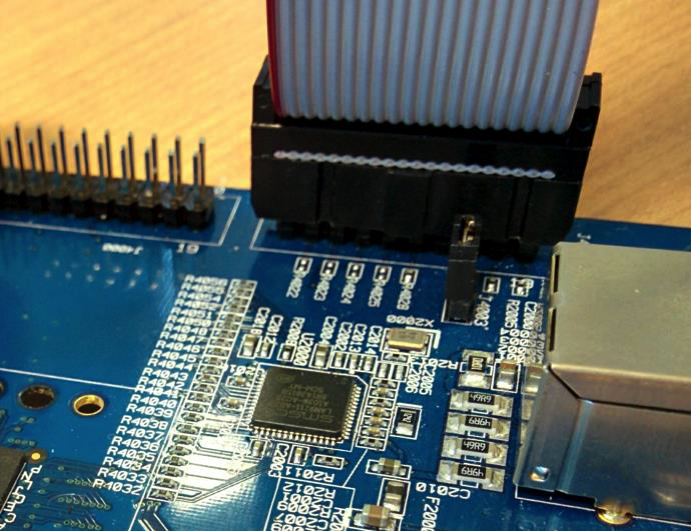
\includegraphics[width=0.35\linewidth]{images/firmware/setup_3}
	\caption{Connection between the STLink/v2 programmer and the SEcubeTM DevKit, close-up (highlighted in red) on the JTAG connector orientation}
	\label{fig:setup3}
\end{figure}


In order to be able to build and flash the firmware, the AC6 Tools must be installed via Eclipse. The AC6 Tool will install the GNU Embedded Toolchain for ARM, which is a ready-to-use, open
source suite of tools for C, C++ and Assembly programming targeting ARM Cortex-M and Cortex-R
family of processors. It includes the GNU Compiler (GCC) and is available free of charge directly
from ARM for embedded so ware development on both Windows and Linux operating systems.
The reference platform for this document is the System Workbench for STM32 (SW4STM32) Eclipse
plugin.

SW4STM32 is an integrated environment that includes:
\begin{itemize}
	\item Building tools (GCC-based ARM cross compiler, assembler and linker);
	\item OpenOCD and GDB debugging tools;
	\item Flash programming tools
\end{itemize}

To install SW4STM32 as an Eclipse plugin:
\begin{enumerate}
	\item launch Eclipse IDE
	\item on the toolbar, click «Help » Install New Software...»
	\item in the Available Software window, click «Add»
	\item in the Add Repository window, set Name and Location fields as follows, and then click «OK»:
	\begin{itemize}
		\item Name: System Workbench for STM32 - Bare Machine edition
		\item Locaton: http://www.ac6-tools.com/Eclipse-updates/org.openstm32.system-workbench.site
	\end{itemize}
	\item select OpenSTM32 Tools and click «Next»
	\item accept the license agreement and click «Finish» to start the plugin installation, continue the installation also if a warning for incompatible or unsigned components is prompted
	\item restart Eclipse
\end{enumerate}



\subsubsection{Firmware flashing}
Once the SECube has been connected to the Host computer via both the ST-Link/v2 programmer and the USB connection, the firmware can be imported, compiled and flashed. 

The latest firmware version has been already compiled and available at ``\textit{SEcube USBStick Firmware/Project/Eclipse/USBStick/Release/USBStick.elf}" but it is possible to import the project into Eclipse and recompile it. If you want to use the pre-compiled version, you can skip the following sections and go to Section \ref{sec:firm_configure}.

In order to import the firmware and the software for performing the init, you need to click «File» and then «Import...», as in Figure \ref{fig:setup6}. At this point after having selected «Existing Projects into Workspace» (Figure \ref{fig:setup7}), the first two projects must be imported (Figure \ref{fig:setup8}).
\begin{figure}[H]
	\centering
	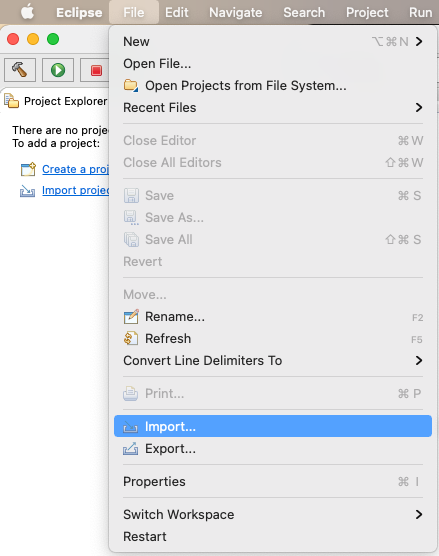
\includegraphics[width=0.35\linewidth]{images/firmware/setup_6}
	\caption{Project import in Eclipse}
	\label{fig:setup6}
\end{figure}
\begin{figure}[H]
	\centering
	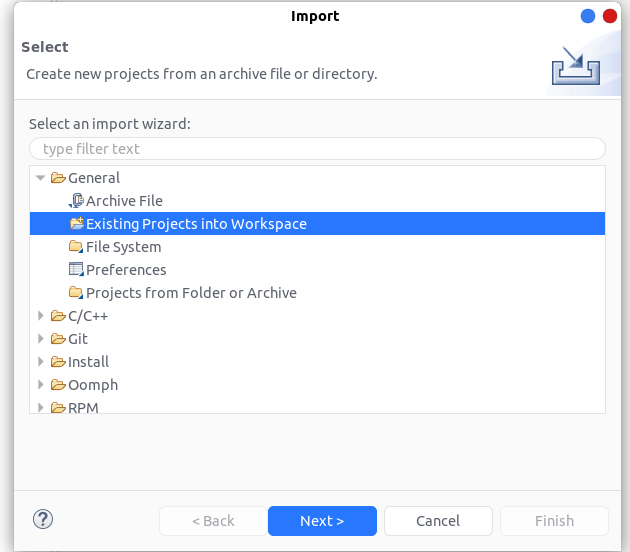
\includegraphics[width=0.55\linewidth]{images/firmware/setup_7}
	\caption{Import of projects}
	\label{fig:setup7}
\end{figure}

\begin{figure}[H]
	\centering
	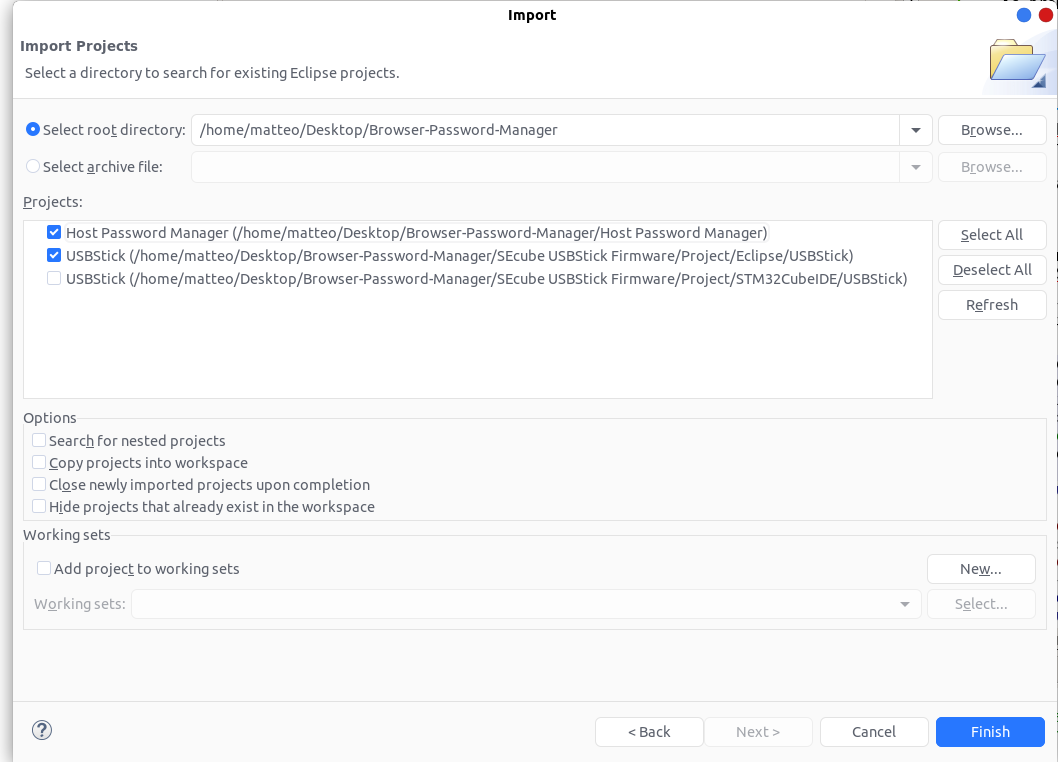
\includegraphics[width=0.55\linewidth]{images/firmware/setup_8}
	\caption{USBStick firmware and Host Password Manager for Initilization}
	\label{fig:setup8}
\end{figure}

The first project will be used during configuration of the device while the second one is the firmware itself.

At this point, on the right you should have two projects, you have to Right click over the ``USBStick" one and select ``Build Project" (refer to Figure \ref{fig:setup10}).
\begin{figure}[H]
	\centering
	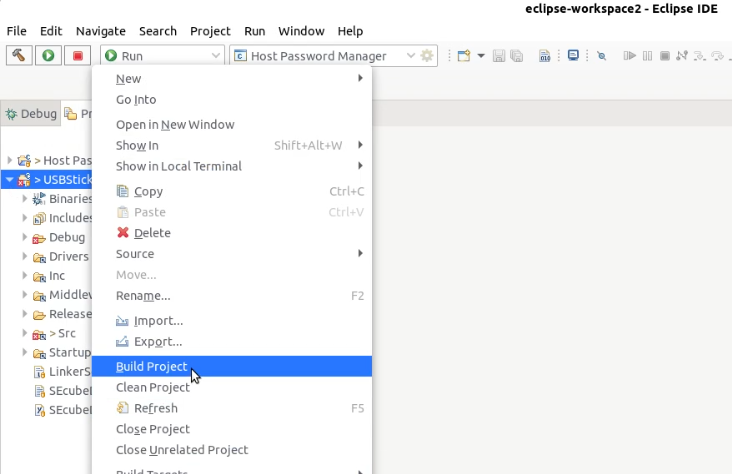
\includegraphics[width=0.55\linewidth]{images/firmware/setup_10}
	\caption{Build the firmware}
	\label{fig:setup10}
\end{figure}

\subsubsection{Configuring the device}
\label{sec:firm_configure}
Once the firmware, you have to first of all to erase the chip in order to remove the previous pin configuration, by doing a Right click on the project and then ``Target" and then ``Erase Chip...". Once it has finished, you can flash the firmware into to the device by clicking ``Target" and then ``Program Chip..." (refer to Figure \ref{fig:setup11}). In the next window you have to select the ``Release" version and flag the ``Reset after program" before clicking ``OK".

\begin{figure}[H]
	\centering
	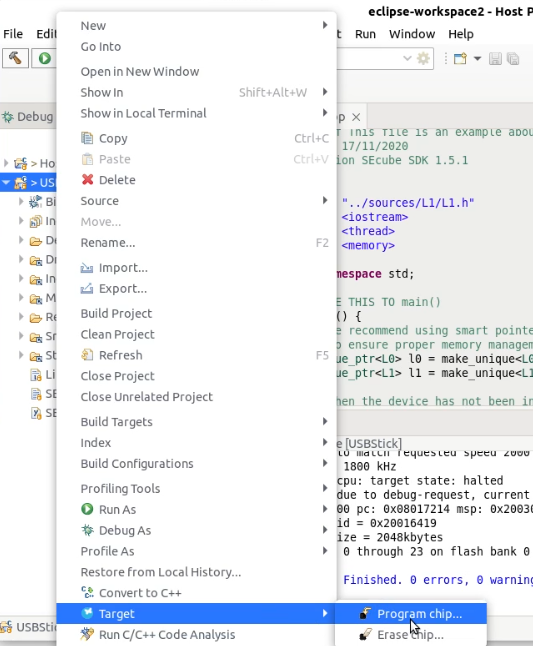
\includegraphics[width=0.55\linewidth]{images/firmware/setup_11}
	\caption{Flash the firmware}
	\label{fig:setup11}
\end{figure}


\begin{figure}[H]
	\centering
	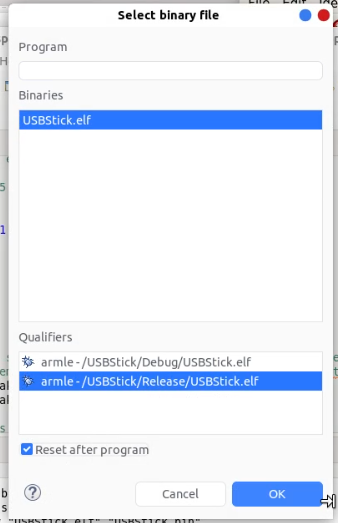
\includegraphics[width=0.3\linewidth]{images/firmware/setup_12}
	\caption{Firmware Release version selection}
	\label{fig:setup12}
\end{figure}

At this point, once the firmware has been flash, you need to configure the device by setting a pin. Now it is the turn of the second project called ``Host Password Manager".\newline\newline
You have to open the \texttt{device\_init.cpp} file and check that the name of the first method is set to \texttt{main}. At this point, you can perform the compilation and run the program. This allows to initialize the device and set the master password for the Secure Password Manager (at line 49 it is possible to change the pin). From now, the device is ready to receive commands by the Host Middleware application in order to manage all passwords features.

\section{Host Middleware}

This section will describe how to build and run the host middleware, both on Linux and Windows. The build process is not necessary because a ready-to-run executable will be provided for the two opearting systems. However, if there are problems in executing them, the build process can be used as a workaround.

\begin{warning}
Because of all the dependencies and operations to achieve a build, some problems may occurr. This section will try to indicate all the necessary eoftware that are required, but unfortunately the successful build of the host middleware is not guaranteed because of the heterogeneous nature of computers.
\end{warning}

\subsection{Linux}
Luckily, on Linux the build process is pretty straightforward. The only thing that needs to be done is to install the necessary software. The following is a list of software that is required to build the host middleware.

\begin{itemize}
    \item \textbf{Python 3.9.x} (tested with 3.9.7). Check that your PATH environment variable points to the Python executable \textit{python3}.
    \item \textbf{pip 20.3.4} (tested with 20.3.4). Check that your PATH environment variable points to the pip executable \textit{pip} and refers to the correct Python version.
    \item \textbf{gcc 11.x} {tested with 11.2.0}. Check that your PATH environment variable points to the gcc executable \textit{gcc}.
    \item \textbf{g++ 11.x} {tested with 11.2.0}. Check that your PATH environment variable points to the g++ executable \textit{g++}.
    \item \textbf{GNU Make} {tested with GNU Make 4.3}. Check that your PATH environment variable points to the GNU Make executable \textit{make}.
    \item \textbf{git} Check that your PATH environment variable points to the git executable \textit{git}.
\end{itemize}

Here a few steps to build the host middleware if all the required software is installed correctly. Note, it can change depending on the used linux distribution. It may requre further steps to install the dependencies.

\begin{lstlisting}[language=bash,caption={bash version}]
$ git clone https://github.com/SEcube-Project/Browser-Password-Manager.git
$ cd Browser-Password-Manager/HostMiddleware

# To build the shared library
$ make clean
$ make -j4 lib.so

# To run the scrypt as-is (include build of lib.so)
$ make clean
$ make -j4 run

# To compile, obfuscate and pack into a single executable
$ make clean
$ make -j4 dist
$ ./BPMMiddleware

\end{lstlisting}


\subsection{Windows}
Unfortunately, on Windows there is a lot more work to do.

\subsubsection{Python}
Python 3.9.x is needed. If you are not sure it's installed on your system, try to launch a Powershell console and type \texttt{python --version}. If you get \texttt{Python 3.9.0} or similar means that Python is installed. Otherwise, you need to install it. \\

\begin{warning}
\textbf{ATTENTION}: if the Windows Store opens up, close it! You need to install it in the \textit{classic way} otherwise strange things will happens later one. 
\end{warning}

\begin{warning}
\textbf{ATTENTION}: if you installed Python from the Windows Store, unistall and download it from \href{https://www.python.org/downloads/release/python-390/}{the official Python webpage}.
\end{warning}

\begin{warning}
\textbf{ATTENTION}: if python is not available from the Powershell after manual installation, try to reboot. If it's still not available, you need to manually specify the Python's executable path. Start menù, type Python, right-click and select "Open File location". Most likely it will head you to the Start Menu Shortcuts, so right-click again on the Python 3.9 folder and click on "Open file location". Select the path and copy in the clipboard. 

In the start menu, search for "environment" and click "Edit the system environment variable". Click on "environment variables" button, select "Path", click "Edit", click "New" and paste the path you previously copied.

Confirm and close everthing, the Powershell too. Open it again and check if now python is available. 
\end{warning}

\subsubsection{C++ Compiler - Buildtools}
Head to the start menù and look for \texttt{x64 Native Tools Command Prompt for VS 2022} (if you are on a 32 bit system, look for \texttt{x86 Native Tools Command Prompt for VS 2022}). Open it, and a terminal emulator will show up. Type \texttt{cl}. If you get \textit{'cl' is not recognized as an internal or external program...} means that something is missing, otherwise you will get the following message and it means that the compiler is installed. Same reasoning must undergo with the \texttt{link} command.

\begin{lstlisting}[language=bash,caption={bash version}]
C:\Program Files\Microsoft Visual Studio\2022\Community>cl
Microsoft (R) C/C++ Optimizing Compiler Version 19.32.31329 for x64
Copyright (C) Microsoft Corporation.  All rights reserved.

usage: cl [ option... ] filename... [ /link linkoption... ]

C:\Program Files\Microsoft Visual Studio\2022\Community>link
Microsoft (R) Incremental Linker Version 14.32.31329.0
Copyright (C) Microsoft Corporation.  All rights reserved.

 usage: LINK [options] [files] [@commandfile]

   options:

      /ALIGN:#
      /ALLOWBIND[:NO]
      /ALLOWISOLATION[:NO]
      /APPCONTAINER[:NO]
      /ASSEMBLYDEBUG[:DISABLE]
      /ASSEMBLYLINKRESOURCE:filename
      /ASSEMBLYMODULE:filename
      /ASSEMBLYRESOURCE:filename[,[name][,PRIVATE]]
      /BASE:{address[,size]|@filename,key}
      /CLRIMAGETYPE:{IJW|PURE|SAFE|SAFE32BITPREFERRED}
      /CLRLOADEROPTIMIZATION:{MD|MDH|NONE|SD}
      /CLRSUPPORTLASTERROR[:{NO|SYSTEMDLL}]
      /CLRTHREADATTRIBUTE:{MTA|NONE|STA}
      /CLRUNMANAGEDCODECHECK[:NO]
      /DEBUG[:{FASTLINK|FULL|NONE}]
      /DEF:filename
      /DEFAULTLIB:library
      /DELAY:{NOBIND|UNLOAD}
      /DELAYLOAD:dll
      /DELAYSIGN[:NO]
      /DEPENDENTLOADFLAG:flag
      /DLL
      /DRIVER[:{UPONLY|WDM}]
      /DYNAMICBASE[:NO]
      /EMITVOLATILEMETADATA[:NO]
(press <return> to continue)

\end{lstlisting}

If something is missing (or the Visual Studio's Command Prompt Tool is not available), Visual Studio must be installed. Go to \href{https://visualstudio.microsoft.com/downloads/}{https://visualstudio.microsoft.com/downloads/} and download Visual Studio Community edition. Once the installer is downloaded, launch it, select \textit{Visual Studio Community 2022} (click on Modify if Visual Studio is already installed) and select \textit{Desktop Development with C++}. The following parts must be installed:

\begin{itemize}
    \item MSVC v143 - VS 2022 C++ x64/x86 build Tools
    \item Windows 10 SDK 
    \item C++/CLI support for v143 build Tools
    \item C++ Modules for v143 build tools
    \item C++ Clang tools for Windows 
\end{itemize}

Repeat from the beginning, be sure that the \textit{Visual Studio's Command Prompt} is installed and the compiler is available. 

\subsubsection{How to build}
Now everything should be installed. Open the Visual Studio's Command Prompt, head to the HostMiddleware folder (with the CD command) and type \texttt{compile\_win.bat}. It will compile everything and pack into a single BPMMiddleware.exe executable that eventually you can run, if everything went fine.\\

Pay attention to antivirus software, it may block the executable. If it does, you can try to disable the antivirus temporarily. Pay attention to use the right Visual Studio's Command Prompt version: if you are on a 64 bit system, use \texttt{x64} instead of \texttt{x86}.\\

If there are problems in packing the executable, you can always try to run directly the python code as-is (under the condition that the dll has been compiled correctly): run \texttt{python app.py}.

\chapter{API}
\label{api}


\section{Host Library L1}
In order to allow to use all functionalities that are provided by the firmware developed for the SECube, the L1 library has been enhanced with additional functions. Even if these methods are used only by the Python Middleware via wrappers, they can be directly used by a custom user Host application.

The following list contains the exhaustive description of all added methods for the Secure Password Manager. Each one of them can be used only after a correct authentication via the L1 \texttt{L1Login} method. All APIs are defined into a custom .cpp file called \texttt{L1\_sepass.cpp} while the signatures are available at \texttt{L1.h}.\newline\newline
Most of the functions are simply used to fill the buffer for the command request and to parse the response, since the application logic has been moved to the firmware itself to increase the security. An example of usage of all the functions below is available at \texttt{examples/manual\_pass\_management.cpp}.

\subsection{Type definition}
In order to simply the interactions with the L1 Secure Password Manager APIs, a custom structure called \texttt{se3Pass} has been defined:
\begin{lstlisting}[language=C++,breaklines=true]
	typedef struct se3Pass_ {
		uint32_t id;
		uint16_t hostSize;
		uint16_t userSize;
		uint16_t passSize;
		std::string host;
		std::string user;
		std::string pass;
	} se3Pass;
\end{lstlisting}

This structure is able to manage as \texttt{string} the hostname, username and password of a Secure Password Manager record. By the way, the total bytes for all fields must not be greater than 4094 byte in total, due to a firmware limitation. This has meaning for both \texttt{L1SEAddPassword} and \texttt{L1SEModifyPassword} methods.\newline\newline
To increase the flexibility of the search functionality, the results can be filtered from the firmware accordingly to:
\begin{itemize}
	\item Hostname
	\item Username
\end{itemize}

For simplicity, an \texttt{enum} creates a correspondence between the numerical value and it's intrinsic information, provided by the name.
\begin{lstlisting}[language=C++,breaklines=true]
	typedef enum se3_list_filter_type_ {
		NO_FILTER = 0,
		HOST_FILTER = 1,
		USER_FILTER = 2
	} se3_list_filter_type;
\end{lstlisting}

\subsection{L1SEGetAllPasswords}
This function exports the list of all passwords in plain text from the SEcube flash memory. In this case, the list is returned as a vector of \texttt{se3Pass} elements. In order to call this function, a vector of type \texttt{se3Pass} must be initialize (e.g. \texttt{std::vector<se3Pass> passList;}).\newline\newline
The function has also a boolean return, that in case of error is set to \texttt{false}.

\begin{lstlisting}[language=C++,breaklines=true]
	bool L1SEGetAllPasswords(std::vector<se3Pass>& passList);
\end{lstlisting}

\subsection{L1SEGetAllPasswordsByUserName}
This function exports the list of all passwords in plain text from the SEcube flash memory filtered by the username, passed as a \texttt{string} parameter. In this case, the list is returned as a vector of \texttt{se3Pass} elements. In order to call this function, a vector of type \texttt{se3Pass} must be initialize (e.g. \texttt{std::vector<se3Pass> passList;}).\newline\newline
The output is the same of the \texttt{L1SEGetAllPasswords} function, but filtered by username.\newline\newline
The function has also a boolean return, that in case of error is set to \texttt{false}.

\begin{lstlisting}[language=C++,breaklines=true]
	bool L1SEGetAllPasswordsByUserName(std::vector<uint8_t> username, std::vector<se3Pass>& passList);
\end{lstlisting}

\subsection{L1SEGetAllPasswordsByHostName}
This function exports the list of all passwords in plain text from the SEcube flash memory filtered by the hostname, passed as a \texttt{string} parameter. In this case, the list is returned as a vector of \texttt{se3Pass} elements. In order to call this function, a vector of type \texttt{se3Pass} must be initialize (e.g. \texttt{std::vector<se3Pass> passList;}).\newline\newline
The output is the same of the \texttt{L1SEGetAllPasswords} function, but filtered by hostname.\newline\newline
The function has also a boolean return, that in case of error is set to \texttt{false}.

\begin{lstlisting}[language=C++,breaklines=true]
	bool L1SEGetAllPasswordsByHostName(std::vector<uint8_t> hostname, std::vector<se3Pass>& passList);
\end{lstlisting}

\subsection{L1SEAddPassword}
The \texttt{L1SEAddPassword} allows to create a new password record by providing:
\begin{itemize}
	\itemsep0sp
	\item ID
	\item Length of the hostname
	\item Length of the username
	\item Length of the password
	\item Hostname
	\item Username
	\item Password
\end{itemize}

\begin{lstlisting}[language=C++,breaklines=true]
	bool L1SEAddPassword(uint16_t pass_id, uint8_t *host_data, uint16_t host_len, uint8_t *user_data, uint16_t user_len, uint8_t *pass_data, uint16_t pass_len);
\end{lstlisting}

The function returns true if the record has been written into the memory of the SECube, in case of error \texttt{false} is returned.

\subsection{L1SEGetPasswordById}
Given a numerical password id, the password record is stored into the \texttt{se3Pass} structure passed as reference. The structure, before calling the method can be initialized as: \texttt{se3Pass searchedById;}.
The function has also a boolean return, that in case of error is set to \texttt{false}.

\begin{lstlisting}[language=C++,breaklines=true]
	bool L1SEGetPasswordById(uint32_t pass_id, se3Pass& password);
\end{lstlisting}

\subsection{L1SEModifyPassword}
Given a numerical password id, the password record is modified accordingly to the new provided \texttt{se3Pass}.
The function has also a boolean return, that in case of error is set to \texttt{false}.
\begin{lstlisting}[language=C++,breaklines=true]
	bool L1SEModifyPassword(uint32_t pass_id, se3Pass& password);
\end{lstlisting}

\subsection{L1SEDeletePassword}
Given a numerical password id, the password with that identified is deleted. If the password is not found or some errors occur, \texttt{false} is returned.
\begin{lstlisting}[language=C++,breaklines=true]
	bool L1SEDeletePassword(uint32_t pass_id);
\end{lstlisting}

\subsection{L1SEGenerateRandomPassword}
Generate a random password with the defined length and with the possibility to include uppercase, special characters and numbers. Via three variables it's possible to enable or disable the presence of a specific character set:
\begin{itemize}
	\itemsep0sp
	\item \texttt{enable\_upper\_case}: uppercase characters
	\item \texttt{enable\_special\_chars}: special characters
	\item \texttt{enable\_numbers\_chars}: symbols
\end{itemize}
The \texttt{pass\_len} parameter allows to define the password dimension, while the result is returned as an array of \texttt{uint8\_t}.

\begin{lstlisting}[language=C++,breaklines=true]
	bool L1SEGenerateRandomPassword(uint16_t pass_len, uint8_t enable_upper_case, uint8_t enable_special_chars, uint8_t enable_numbers_chars, std::shared_ptr<uint8_t[]> generated_pass);
\end{lstlisting}

It's important to mention that all the complexity of the generation is moved into the SECube to increase the security. Moreover, if a character set is selected, at least one char of that type must be included into the output random password.



\section{Middleware HTTPs' API}

\subsection{/api/v0/time}
Used to work with the timestamp. The timestamp is an integer in seconds. The supported HTTP methods are:

\begin{itemize}
    \item \texttt{GET}: returns the current timestamp.
\end{itemize}

\subsection{/api/v0/devices}
Used to work with the devices. It allows to obtain all the connected boards, in particular for each device the ID, Name and Serial are returned. The API is currently not used by the Extension because it' supposed that only one device at a time is connected. The supported HTTP methods are:

\begin{itemize}
    \item \texttt{GET}: returns the list of devices.
\end{itemize}

\subsection{/api/v0/device/\{id\}/sessions}
Used to manage sessions. The supported HTTP methods are:

\begin{itemize}
    \item \texttt{GET}: allow to know if the cookie attached to the request represents a valid session or not.
    \item \texttt{POST}: creates a new session. The \textit{PIN} and the \textit{timestamp} parameters are mandatory. The \textit{timestamp} parameter is an integer in seconds.
    \item \texttt{DELETE}: forces to invalidate the session attached to the cookie.
\end{itemize}

\subsection{/api/v0/device/\{id\}/generate}
Used to generate a new password using the exposed funcionality of the board. The supported HTTP methods are:

\begin{itemize}
    \item \texttt{GET}: allows to obtain a new randomly generated password. The optional parameters are:
        \subitem \texttt{length}: the length of the password. The default value is 64.
        \subitem \texttt{upper}: boolean value that indicates if the password must contain uppercase letters. The default value is 1. Can be 0.
        \subitem \texttt{special}: boolean value that indicates if the password must contain special characters. The default value is 1. Can be 0.
        \subitem \texttt{numbers}: boolean value that indicates if the password must contain numeric characters. The default value is 1. Can be 0.
\end{itemize}

\subsection{/api/v0/device/\{id\}/passwords}
Used to manage passwords. The supported HTTP methods are:

\begin{itemize}
    \item \texttt{GET}: allows to obtain the list of passwords. It supports the \texttt{hostname} parameter to filter the list of passwords by hostname. The \texttt{hostname} parameter is a string. Each password is represented by a JSON object with the following fields:
        \subitem \texttt{hostname}: the hostname of the password.
        \subitem \texttt{password}: the password.
        \subitem \texttt{username}: the username.
        \subitem \texttt{id}: the ID of the password.
    \item \texttt{POST}: allows to add and store in the board a new password. The parameters must be passed via the body in the form of a JSON object. The mandatory parameters are:
        \subitem \texttt{hostname}: the hostname of the password.
        \subitem \texttt{password}: the password.
        \subitem \texttt{username}: the username.
\end{itemize}

\subsection{/api/v0/device/\{id\}/password/\{id\}}
Allows to manage a single password. The supported HTTP methods are:

\begin{itemize}
    \item \texttt{GET}: allows to obtain the password record. The password is represented by a JSON object with the following fields:
        \subitem \texttt{hostname}: the hostname of the password.
        \subitem \texttt{password}: the password.
        \subitem \texttt{username}: the username.
        \subitem \texttt{id}: the ID of the password.
    \item \texttt{DELETE}: allows to delete the password.
    \item \texttt{PUT}: allows to update the password. The parameters must be passed via the body in the form of a JSON object, as the one to add a new password. The mandatory parameters are:
        \subitem \texttt{hostname}: the hostname of the password.
        \subitem \texttt{password}: the password.
        \subitem \texttt{username}: the username.
\end{itemize}

%%%%%%%%%%%%%%%%%%%%%%%%%%%%%%%%%%%%%%%%%%%%%%%%%%%%%

\end{document}